\documentclass{book}

\title{VCSBeam Documentation}
\author{Dr. Sammy McSweeney}

\usepackage{amsmath}
\usepackage{fullpage}
\usepackage{listings}
\usepackage{graphicx}
\usepackage{hyperref}
\usepackage{natbib}

\begin{document}

\maketitle

\tableofcontents

\chapter{Conventions}

\section{Coordinate systems}

There are three coordinate systems in use throughout VCSBeam:
\begin{enumerate}
    \item Instrumental
    \item Sky (local coordinates)
    \item Sky (celestial coordinates)
\end{enumerate}
They are illustrated in Fig. \ref{fig:coords}.
\begin{figure}[!bh]
    \centering
    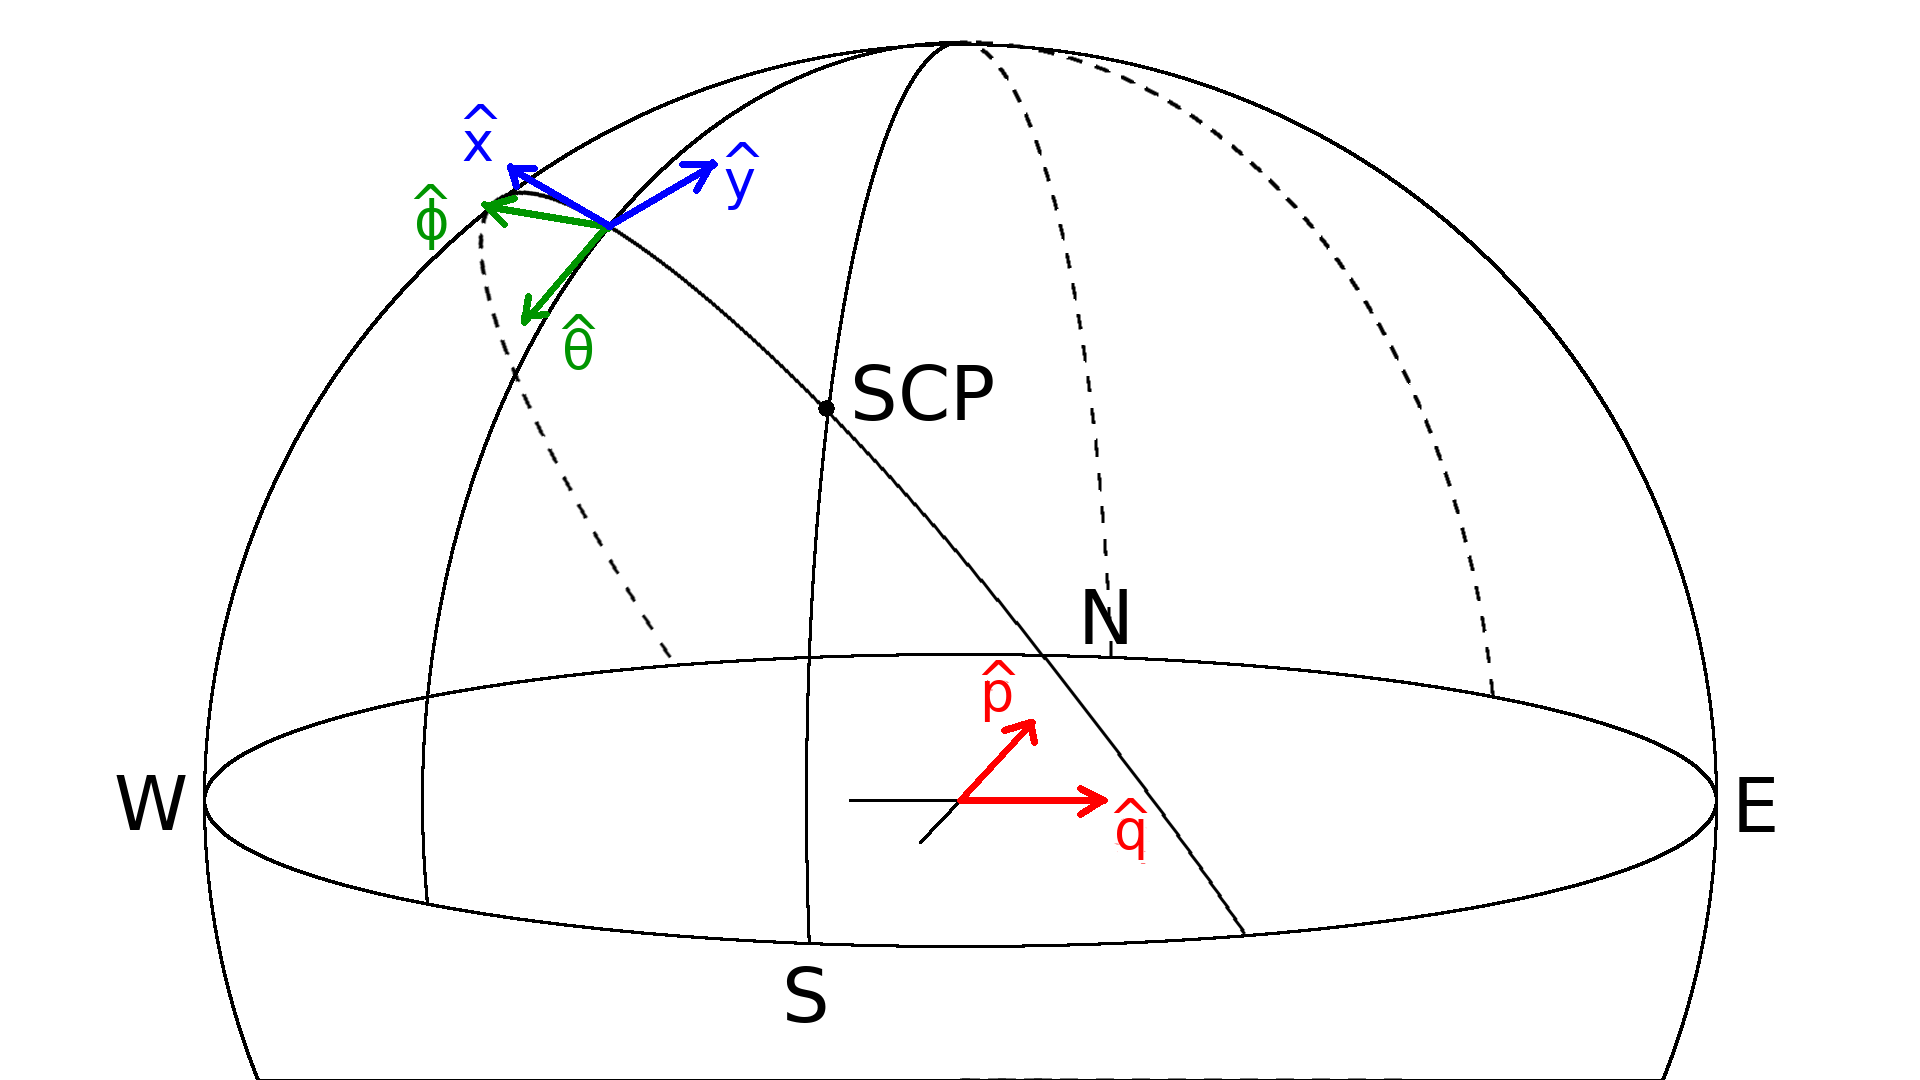
\includegraphics[width=\textwidth]{coords.png}
    \caption{Illustration of the three coordinate systems used in this work\dots}
    \label{fig:coords}
\end{figure}

\subsection{Notation in other documents}

See Table \ref{tbl:notations}
\begin{table}[!hb]
    \centering
    \caption{Comparison of notation used elsewhere}
    \label{tbl:notations}
    \begin{tabular}{l|cc|cc|cc}
        & P & Q & $\theta$ & $\phi$ & X & Y \\
        \hline
        MWA metafits files       & Y & X & - & - & - & - \\
        Sokolowksi et al. (2017) & $y$ & $x$ & $\theta$ & $\phi$ & - & - \\
    \end{tabular}
\end{table}

\chapter{PFB}

\section{Fine channelisation}

\chapter{Calibration}

\section{RTS}

\chapter{Beamforming}

\chapter{Applications}

\chapter{Utilities}


\end{document}
